\documentclass[]{article}
\usepackage{lmodern}
\usepackage{amssymb,amsmath}
\usepackage{ifxetex,ifluatex}
\usepackage{fixltx2e} % provides \textsubscript
\ifnum 0\ifxetex 1\fi\ifluatex 1\fi=0 % if pdftex
  \usepackage[T1]{fontenc}
  \usepackage[utf8]{inputenc}
\else % if luatex or xelatex
  \ifxetex
    \usepackage{mathspec}
  \else
    \usepackage{fontspec}
  \fi
  \defaultfontfeatures{Ligatures=TeX,Scale=MatchLowercase}
\fi
% use upquote if available, for straight quotes in verbatim environments
\IfFileExists{upquote.sty}{\usepackage{upquote}}{}
% use microtype if available
\IfFileExists{microtype.sty}{%
\usepackage{microtype}
\UseMicrotypeSet[protrusion]{basicmath} % disable protrusion for tt fonts
}{}
\usepackage[margin=1in]{geometry}
\usepackage{hyperref}
\hypersetup{unicode=true,
            pdftitle={M\&E plots in ggplot2},
            pdfauthor={Nathan Green, Imperial College London},
            pdfborder={0 0 0},
            breaklinks=true}
\urlstyle{same}  % don't use monospace font for urls
\usepackage{color}
\usepackage{fancyvrb}
\newcommand{\VerbBar}{|}
\newcommand{\VERB}{\Verb[commandchars=\\\{\}]}
\DefineVerbatimEnvironment{Highlighting}{Verbatim}{commandchars=\\\{\}}
% Add ',fontsize=\small' for more characters per line
\usepackage{framed}
\definecolor{shadecolor}{RGB}{248,248,248}
\newenvironment{Shaded}{\begin{snugshade}}{\end{snugshade}}
\newcommand{\AlertTok}[1]{\textcolor[rgb]{0.94,0.16,0.16}{#1}}
\newcommand{\AnnotationTok}[1]{\textcolor[rgb]{0.56,0.35,0.01}{\textbf{\textit{#1}}}}
\newcommand{\AttributeTok}[1]{\textcolor[rgb]{0.77,0.63,0.00}{#1}}
\newcommand{\BaseNTok}[1]{\textcolor[rgb]{0.00,0.00,0.81}{#1}}
\newcommand{\BuiltInTok}[1]{#1}
\newcommand{\CharTok}[1]{\textcolor[rgb]{0.31,0.60,0.02}{#1}}
\newcommand{\CommentTok}[1]{\textcolor[rgb]{0.56,0.35,0.01}{\textit{#1}}}
\newcommand{\CommentVarTok}[1]{\textcolor[rgb]{0.56,0.35,0.01}{\textbf{\textit{#1}}}}
\newcommand{\ConstantTok}[1]{\textcolor[rgb]{0.00,0.00,0.00}{#1}}
\newcommand{\ControlFlowTok}[1]{\textcolor[rgb]{0.13,0.29,0.53}{\textbf{#1}}}
\newcommand{\DataTypeTok}[1]{\textcolor[rgb]{0.13,0.29,0.53}{#1}}
\newcommand{\DecValTok}[1]{\textcolor[rgb]{0.00,0.00,0.81}{#1}}
\newcommand{\DocumentationTok}[1]{\textcolor[rgb]{0.56,0.35,0.01}{\textbf{\textit{#1}}}}
\newcommand{\ErrorTok}[1]{\textcolor[rgb]{0.64,0.00,0.00}{\textbf{#1}}}
\newcommand{\ExtensionTok}[1]{#1}
\newcommand{\FloatTok}[1]{\textcolor[rgb]{0.00,0.00,0.81}{#1}}
\newcommand{\FunctionTok}[1]{\textcolor[rgb]{0.00,0.00,0.00}{#1}}
\newcommand{\ImportTok}[1]{#1}
\newcommand{\InformationTok}[1]{\textcolor[rgb]{0.56,0.35,0.01}{\textbf{\textit{#1}}}}
\newcommand{\KeywordTok}[1]{\textcolor[rgb]{0.13,0.29,0.53}{\textbf{#1}}}
\newcommand{\NormalTok}[1]{#1}
\newcommand{\OperatorTok}[1]{\textcolor[rgb]{0.81,0.36,0.00}{\textbf{#1}}}
\newcommand{\OtherTok}[1]{\textcolor[rgb]{0.56,0.35,0.01}{#1}}
\newcommand{\PreprocessorTok}[1]{\textcolor[rgb]{0.56,0.35,0.01}{\textit{#1}}}
\newcommand{\RegionMarkerTok}[1]{#1}
\newcommand{\SpecialCharTok}[1]{\textcolor[rgb]{0.00,0.00,0.00}{#1}}
\newcommand{\SpecialStringTok}[1]{\textcolor[rgb]{0.31,0.60,0.02}{#1}}
\newcommand{\StringTok}[1]{\textcolor[rgb]{0.31,0.60,0.02}{#1}}
\newcommand{\VariableTok}[1]{\textcolor[rgb]{0.00,0.00,0.00}{#1}}
\newcommand{\VerbatimStringTok}[1]{\textcolor[rgb]{0.31,0.60,0.02}{#1}}
\newcommand{\WarningTok}[1]{\textcolor[rgb]{0.56,0.35,0.01}{\textbf{\textit{#1}}}}
\usepackage{graphicx,grffile}
\makeatletter
\def\maxwidth{\ifdim\Gin@nat@width>\linewidth\linewidth\else\Gin@nat@width\fi}
\def\maxheight{\ifdim\Gin@nat@height>\textheight\textheight\else\Gin@nat@height\fi}
\makeatother
% Scale images if necessary, so that they will not overflow the page
% margins by default, and it is still possible to overwrite the defaults
% using explicit options in \includegraphics[width, height, ...]{}
\setkeys{Gin}{width=\maxwidth,height=\maxheight,keepaspectratio}
\IfFileExists{parskip.sty}{%
\usepackage{parskip}
}{% else
\setlength{\parindent}{0pt}
\setlength{\parskip}{6pt plus 2pt minus 1pt}
}
\setlength{\emergencystretch}{3em}  % prevent overfull lines
\providecommand{\tightlist}{%
  \setlength{\itemsep}{0pt}\setlength{\parskip}{0pt}}
\setcounter{secnumdepth}{0}
% Redefines (sub)paragraphs to behave more like sections
\ifx\paragraph\undefined\else
\let\oldparagraph\paragraph
\renewcommand{\paragraph}[1]{\oldparagraph{#1}\mbox{}}
\fi
\ifx\subparagraph\undefined\else
\let\oldsubparagraph\subparagraph
\renewcommand{\subparagraph}[1]{\oldsubparagraph{#1}\mbox{}}
\fi

%%% Use protect on footnotes to avoid problems with footnotes in titles
\let\rmarkdownfootnote\footnote%
\def\footnote{\protect\rmarkdownfootnote}

%%% Change title format to be more compact
\usepackage{titling}

% Create subtitle command for use in maketitle
\providecommand{\subtitle}[1]{
  \posttitle{
    \begin{center}\large#1\end{center}
    }
}

\setlength{\droptitle}{-2em}

  \title{M\&E plots in ggplot2}
    \pretitle{\vspace{\droptitle}\centering\huge}
  \posttitle{\par}
    \author{Nathan Green, Imperial College London}
    \preauthor{\centering\large\emph}
  \postauthor{\par}
      \predate{\centering\large\emph}
  \postdate{\par}
    \date{07/09/2019}


\begin{document}
\maketitle

\hypertarget{distribution-of-afp-cases-by-month-pakistan-2015-2019}{%
\subsubsection{Distribution of AFP Cases by Month, Pakistan
2015-2019}\label{distribution-of-afp-cases-by-month-pakistan-2015-2019}}

Read in the required packages.

\begin{Shaded}
\begin{Highlighting}[]
\KeywordTok{library}\NormalTok{(dplyr)}
\end{Highlighting}
\end{Shaded}

\begin{verbatim}
## Warning: package 'dplyr' was built under R version 3.5.3
\end{verbatim}

\begin{verbatim}
## 
## Attaching package: 'dplyr'
\end{verbatim}

\begin{verbatim}
## The following objects are masked from 'package:stats':
## 
##     filter, lag
\end{verbatim}

\begin{verbatim}
## The following objects are masked from 'package:base':
## 
##     intersect, setdiff, setequal, union
\end{verbatim}

\begin{Shaded}
\begin{Highlighting}[]
\KeywordTok{library}\NormalTok{(ggplot2)}
\end{Highlighting}
\end{Shaded}

\begin{verbatim}
## Warning: package 'ggplot2' was built under R version 3.5.3
\end{verbatim}

\begin{Shaded}
\begin{Highlighting}[]
\KeywordTok{library}\NormalTok{(lubridate)}
\end{Highlighting}
\end{Shaded}

\begin{verbatim}
## Warning: package 'lubridate' was built under R version 3.5.3
\end{verbatim}

\begin{verbatim}
## 
## Attaching package: 'lubridate'
\end{verbatim}

\begin{verbatim}
## The following object is masked from 'package:base':
## 
##     date
\end{verbatim}

Read in data from Excel file
\texttt{List\ of\ AFP\ Cases\ 2015-2019.xlsx}.

\begin{Shaded}
\begin{Highlighting}[]
\KeywordTok{library}\NormalTok{(dataPakistan)}

\NormalTok{file_name <-}\StringTok{ }\KeywordTok{system.file}\NormalTok{(}\DataTypeTok{package =} \StringTok{"dataPakistan"}\NormalTok{, }\StringTok{"extdata"}\NormalTok{, }\StringTok{"List of AFP Cases 2015-2019.xlsx"}\NormalTok{)}
\NormalTok{dat <-}\StringTok{ }\NormalTok{readxl}\OperatorTok{::}\KeywordTok{read_xlsx}\NormalTok{(file_name, }\DataTypeTok{sheet =} \StringTok{"Data"}\NormalTok{)}
\end{Highlighting}
\end{Shaded}

\begin{Shaded}
\begin{Highlighting}[]
\CommentTok{##############}
\CommentTok{# preprocess #}
\CommentTok{##############}

\CommentTok{# extract only the month from the date in `DENTER`}
\NormalTok{dat}\OperatorTok{$}\NormalTok{month <-}\StringTok{ }\NormalTok{lubridate}\OperatorTok{::}\KeywordTok{month}\NormalTok{(dat}\OperatorTok{$}\NormalTok{DENTER, }\DataTypeTok{label =} \OtherTok{TRUE}\NormalTok{)}

\CommentTok{# create a new column called `afp_cases` that is `TRUE` is `ALL DIAGNOSED` is recorded in `AFP`}
\NormalTok{dat}\OperatorTok{$}\NormalTok{afp_cases <-}\StringTok{ }\NormalTok{dat}\OperatorTok{$}\NormalTok{AFP }\OperatorTok{==}\StringTok{ "ALL DIAGNOSED"}
\end{Highlighting}
\end{Shaded}

We're going to use the \texttt{dplyr} package functions to take
aggregate statistics for months and years on onset.

\begin{Shaded}
\begin{Highlighting}[]
\NormalTok{x <-}
\StringTok{  }\NormalTok{dat }\OperatorTok\StringTok{ }
\StringTok{  }\KeywordTok{group_by}\NormalTok{(month, YRONSET) }\OperatorTok\StringTok{                           }\CommentTok{# separate the data set in to subsets of each month and year of onset}
\StringTok{  }\KeywordTok{summarise}\NormalTok{(}\DataTypeTok{cases =} \KeywordTok{sum}\NormalTok{(afp_cases, }\DataTypeTok{na.rm =} \OtherTok{TRUE}\NormalTok{)) }\OperatorTok\StringTok{    }\CommentTok{# within each of these subgroups calculate the sum total of `afp_cases`}
\StringTok{  }\KeywordTok{mutate}\NormalTok{(}\DataTypeTok{month_year =} \KeywordTok{paste}\NormalTok{(month, YRONSET)) }\OperatorTok\StringTok{         }\CommentTok{# create a new column coombining month and year of onset into a single character string}
\StringTok{  }\KeywordTok{arrange}\NormalTok{(YRONSET, month)                                }\CommentTok{# sort the rows by increasing year of onset and then month}
\end{Highlighting}
\end{Shaded}

\begin{Shaded}
\begin{Highlighting}[]
\CommentTok{#########}
\CommentTok{# plots #}
\CommentTok{#########}


\CommentTok{# basic base R bar plot}

\KeywordTok{barplot}\NormalTok{(}\DataTypeTok{height =}\NormalTok{ x}\OperatorTok{$}\NormalTok{cases,}
        \DataTypeTok{col =} \StringTok{"darkgreen"}\NormalTok{,   }\CommentTok{# colour the bars }
        \DataTypeTok{names.arg =}\NormalTok{ x}\OperatorTok{$}\NormalTok{month, }\CommentTok{# labels on the x-axis}
        \DataTypeTok{las =} \DecValTok{2}\NormalTok{)             }\CommentTok{# resize the axis labels}

\CommentTok{# Annotate the x-axis with the year 2015 to 2019}
\KeywordTok{mtext}\NormalTok{(}\StringTok{"2015"}\NormalTok{, }\DataTypeTok{side =} \DecValTok{1}\NormalTok{, }\DataTypeTok{line =} \DecValTok{3}\NormalTok{, }\DataTypeTok{at =} \DecValTok{8}\NormalTok{)}
\KeywordTok{mtext}\NormalTok{(}\StringTok{"2016"}\NormalTok{, }\DataTypeTok{side =} \DecValTok{1}\NormalTok{, }\DataTypeTok{line =} \DecValTok{3}\NormalTok{, }\DataTypeTok{at =} \DecValTok{22}\NormalTok{)}
\KeywordTok{mtext}\NormalTok{(}\StringTok{"2017"}\NormalTok{, }\DataTypeTok{side =} \DecValTok{1}\NormalTok{, }\DataTypeTok{line =} \DecValTok{3}\NormalTok{, }\DataTypeTok{at =} \DecValTok{36}\NormalTok{)}
\KeywordTok{mtext}\NormalTok{(}\StringTok{"2018"}\NormalTok{, }\DataTypeTok{side =} \DecValTok{1}\NormalTok{, }\DataTypeTok{line =} \DecValTok{3}\NormalTok{, }\DataTypeTok{at =} \DecValTok{50}\NormalTok{)}
\KeywordTok{mtext}\NormalTok{(}\StringTok{"2019"}\NormalTok{, }\DataTypeTok{side =} \DecValTok{1}\NormalTok{, }\DataTypeTok{line =} \DecValTok{3}\NormalTok{, }\DataTypeTok{at =} \DecValTok{64}\NormalTok{)}

\KeywordTok{title}\NormalTok{(}\DataTypeTok{main =} \StringTok{"Graph 1:Distribution of AFP Cases by Month, Pakistan 2015-2019*"}\NormalTok{,}
      \DataTypeTok{ylab =} \StringTok{"Cases (n)"}\NormalTok{)}

\CommentTok{# add vertical lines at given times}
\KeywordTok{abline}\NormalTok{(}\DataTypeTok{v =} \DecValTok{15}\NormalTok{)}
\KeywordTok{abline}\NormalTok{(}\DataTypeTok{v =} \DecValTok{30}\NormalTok{)}
\KeywordTok{abline}\NormalTok{(}\DataTypeTok{v =} \DecValTok{45}\NormalTok{)}
\end{Highlighting}
\end{Shaded}

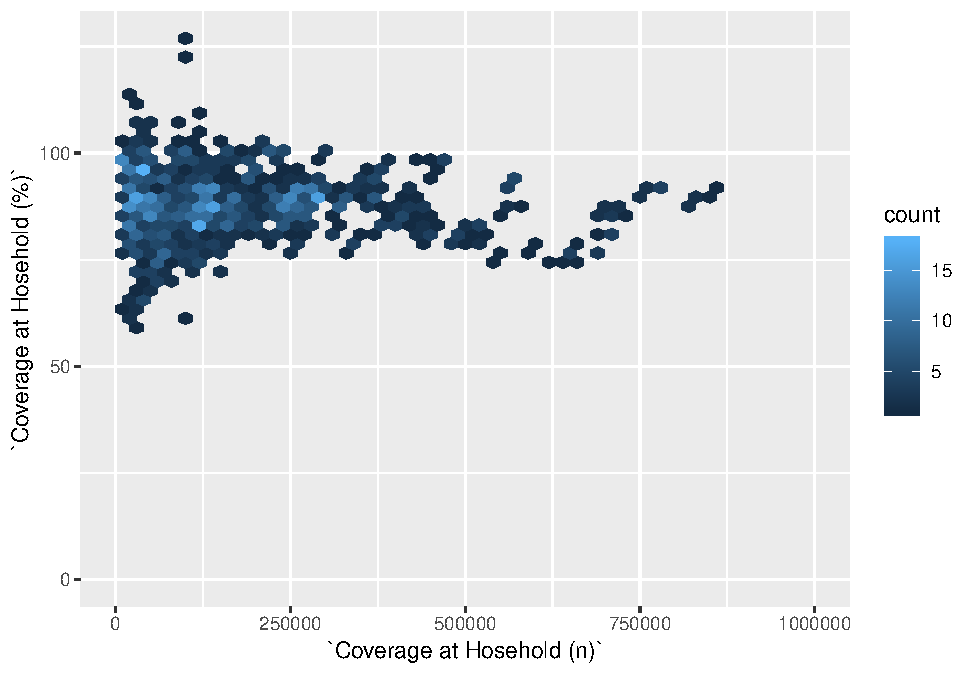
\includegraphics{M_E-plots-in-ggplot2_files/figure-latex/unnamed-chunk-5-1.pdf}

\begin{Shaded}
\begin{Highlighting}[]
\CommentTok{# ggplot version}

\CommentTok{# basic ggplot bar plot}
\NormalTok{plot0 <-}
\StringTok{  }\KeywordTok{ggplot}\NormalTok{(x, }\KeywordTok{aes}\NormalTok{(}\DataTypeTok{x =}\NormalTok{ month_year, }\DataTypeTok{y =}\NormalTok{ cases)) }\OperatorTok{+}
\StringTok{  }\KeywordTok{geom_bar}\NormalTok{(}\DataTypeTok{stat =} \StringTok{"identity"}\NormalTok{)}

\NormalTok{plot0}
\end{Highlighting}
\end{Shaded}

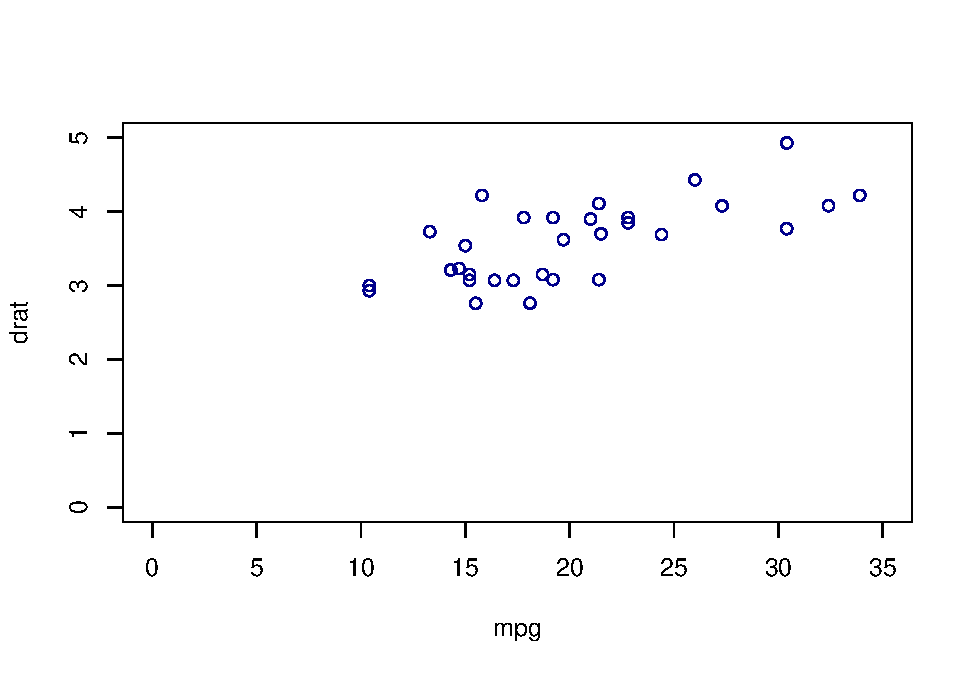
\includegraphics{M_E-plots-in-ggplot2_files/figure-latex/unnamed-chunk-6-1.pdf}

What are the thinks wrong with this?

Firstly, the order of the months is not in calendar order but
alphabetical so we can reorder how they are plotted by using
\texttt{levels} in \texttt{factor}.

\begin{Shaded}
\begin{Highlighting}[]
\NormalTok{x}\OperatorTok{$}\NormalTok{month <-}\StringTok{ }\KeywordTok{factor}\NormalTok{(x}\OperatorTok{$}\NormalTok{month, }\DataTypeTok{ordered =} \OtherTok{TRUE}\NormalTok{)}
\NormalTok{x}\OperatorTok{$}\NormalTok{month_year <-}\StringTok{ }\KeywordTok{factor}\NormalTok{(x}\OperatorTok{$}\NormalTok{month_year, }\DataTypeTok{levels =}\NormalTok{ x}\OperatorTok{$}\NormalTok{month_year, }\DataTypeTok{ordered =} \OtherTok{TRUE}\NormalTok{)}

\NormalTok{plot0 <-}
\StringTok{  }\KeywordTok{ggplot}\NormalTok{(x, }\KeywordTok{aes}\NormalTok{(}\DataTypeTok{x =}\NormalTok{ month_year, }\DataTypeTok{y =}\NormalTok{ cases)) }\OperatorTok{+}
\StringTok{  }\KeywordTok{geom_bar}\NormalTok{(}\DataTypeTok{stat =} \StringTok{"identity"}\NormalTok{)}

\NormalTok{plot0}
\end{Highlighting}
\end{Shaded}

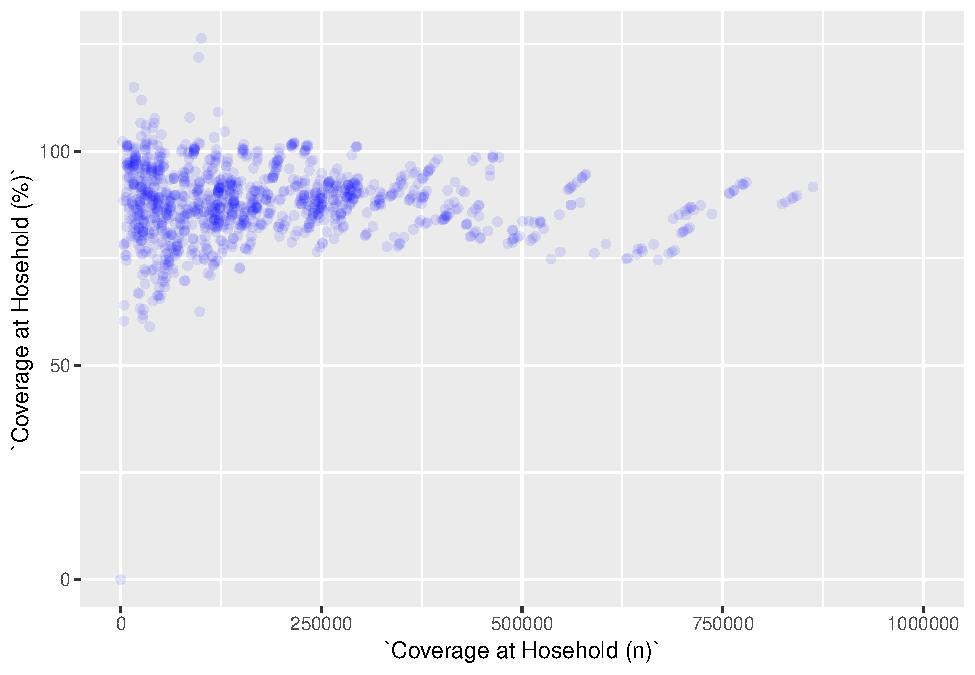
\includegraphics{M_E-plots-in-ggplot2_files/figure-latex/unnamed-chunk-7-1.pdf}

Lets rename the axis labels.

\begin{Shaded}
\begin{Highlighting}[]
\NormalTok{plot1 <-}
\StringTok{  }\NormalTok{plot0 }\OperatorTok{+}
\StringTok{  }\KeywordTok{xlab}\NormalTok{(}\StringTok{""}\NormalTok{) }\OperatorTok{+}
\StringTok{  }\KeywordTok{ylab}\NormalTok{(}\StringTok{"Cases (n)"}\NormalTok{)}

\NormalTok{plot1}
\end{Highlighting}
\end{Shaded}

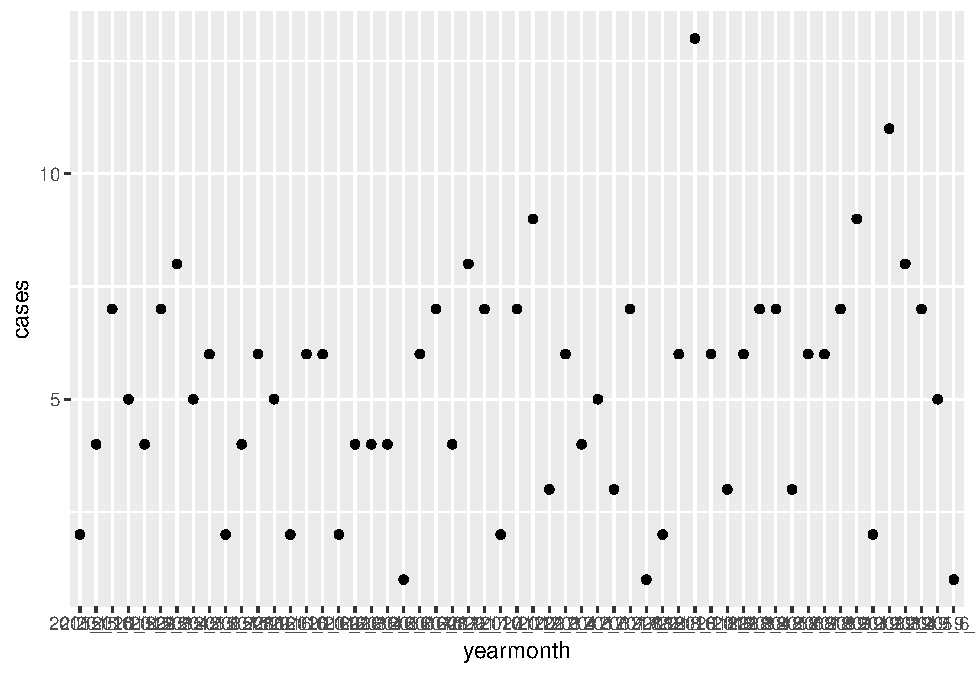
\includegraphics{M_E-plots-in-ggplot2_files/figure-latex/unnamed-chunk-8-1.pdf}

Now make some space around the edges of the plot

\begin{Shaded}
\begin{Highlighting}[]
\NormalTok{plot2 <-}
\StringTok{  }\NormalTok{plot1 }\OperatorTok{+}\StringTok{ }
\StringTok{  }\KeywordTok{scale_x_discrete}\NormalTok{(}\DataTypeTok{breaks =}\NormalTok{ x}\OperatorTok{$}\NormalTok{month_year, }\DataTypeTok{labels =}\NormalTok{ x}\OperatorTok{$}\NormalTok{month,}
                   \DataTypeTok{expand =} \KeywordTok{c}\NormalTok{(}\FloatTok{0.1}\NormalTok{,}\FloatTok{0.1}\NormalTok{))}
\NormalTok{plot2}
\end{Highlighting}
\end{Shaded}

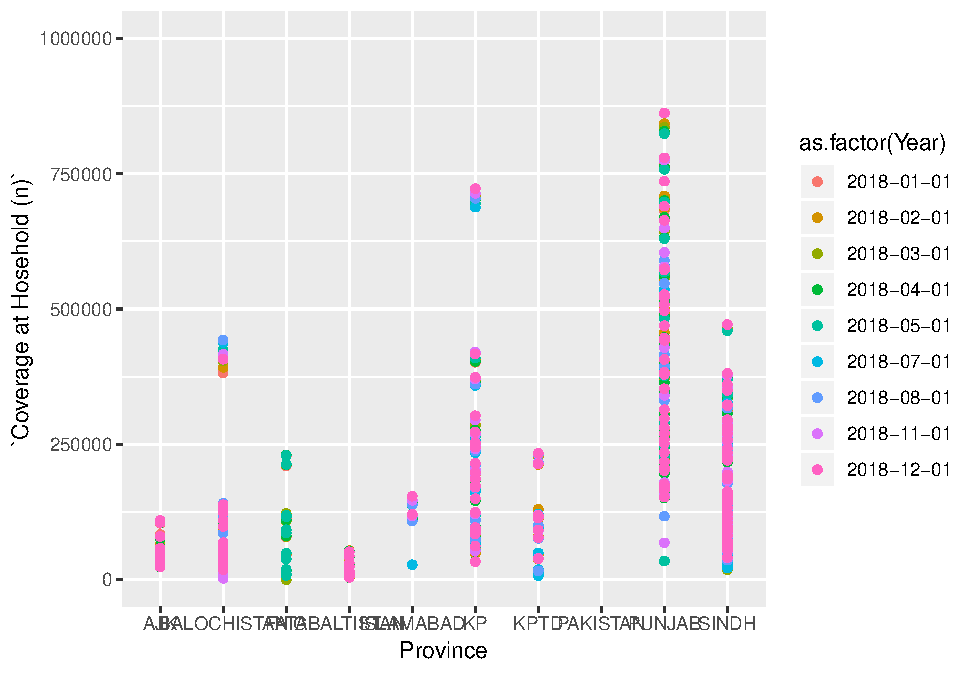
\includegraphics{M_E-plots-in-ggplot2_files/figure-latex/unnamed-chunk-9-1.pdf}

We want to make it clear which months are from which year by adding some
space between years and labelling.

\begin{Shaded}
\begin{Highlighting}[]
\NormalTok{plot3 <-}\StringTok{ }
\StringTok{  }\NormalTok{plot2 }\OperatorTok{+}
\StringTok{  }\KeywordTok{facet_grid}\NormalTok{(}\OperatorTok{~}\StringTok{ }\NormalTok{YRONSET, }\DataTypeTok{space =} \StringTok{"free_x"}\NormalTok{, }\DataTypeTok{scales =} \StringTok{"free_x"}\NormalTok{, }\DataTypeTok{switch =} \StringTok{"x"}\NormalTok{)}

\NormalTok{plot3}
\end{Highlighting}
\end{Shaded}

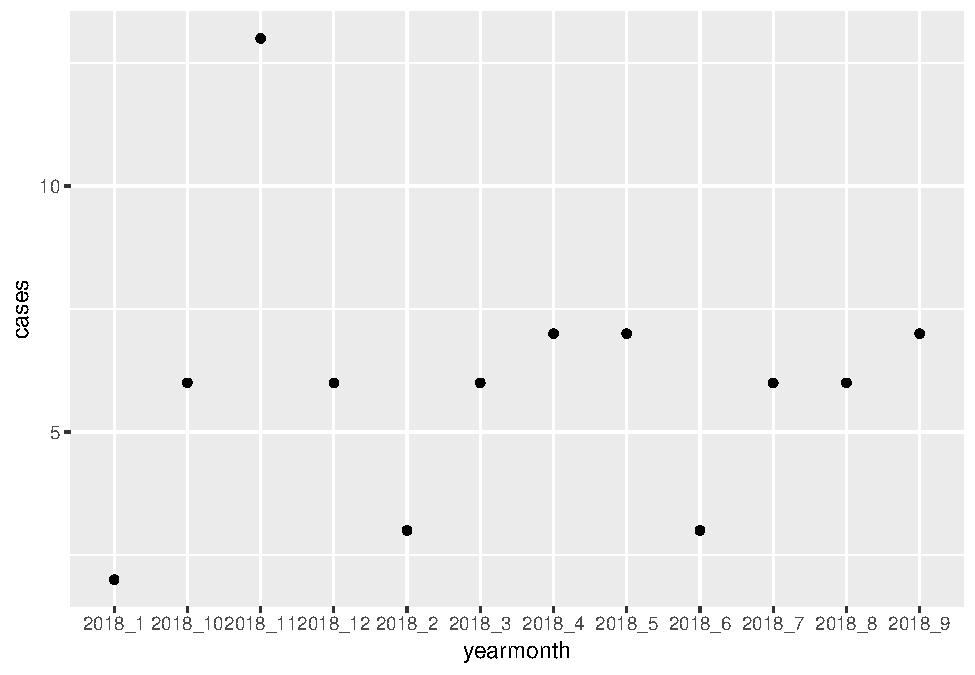
\includegraphics{M_E-plots-in-ggplot2_files/figure-latex/unnamed-chunk-10-1.pdf}

Now we have the basic layout of the plot, we want to edit the style.
From the example we were given there are several small asthetic changes
we can make by using \texttt{theme()}.

\begin{Shaded}
\begin{Highlighting}[]
\NormalTok{plot4 <-}\StringTok{ }
\StringTok{  }\NormalTok{plot3 }\OperatorTok{+}\StringTok{ }
\StringTok{  }\KeywordTok{theme_bw}\NormalTok{() }\OperatorTok{+}\StringTok{                                                                      }\CommentTok{# use a black and white theme}
\StringTok{  }\KeywordTok{ggtitle}\NormalTok{(}\StringTok{"Graph 1:Distribution of AFP Cases by Month, Pakistan 2015-2019*"}\NormalTok{) }\OperatorTok{+}
\StringTok{  }\KeywordTok{theme}\NormalTok{(}\DataTypeTok{strip.placement =} \StringTok{"outside"}\NormalTok{,                                    }\CommentTok{# swap the year and months labels on the x-axis}
        \DataTypeTok{strip.background =} \KeywordTok{element_rect}\NormalTok{(}\DataTypeTok{fill =} \OtherTok{NA}\NormalTok{, }\DataTypeTok{colour =} \StringTok{"green"}\NormalTok{),   }\CommentTok{# change background & border colour of year labels}
        \DataTypeTok{panel.spacing =} \KeywordTok{unit}\NormalTok{(}\DecValTok{0}\NormalTok{,}\StringTok{"cm"}\NormalTok{),                                  }\CommentTok{# reduce the spacing between years}
        \DataTypeTok{panel.grid.major.x =} \KeywordTok{element_line}\NormalTok{(}\DataTypeTok{colour =} \OtherTok{NA}\NormalTok{, }\DataTypeTok{size =} \OtherTok{NULL}\NormalTok{, }\DataTypeTok{linetype =} \OtherTok{NULL}\NormalTok{,  }\CommentTok{# remove x and y grid lines}
                                          \DataTypeTok{lineend =} \OtherTok{NULL}\NormalTok{, }\DataTypeTok{color =} \OtherTok{NULL}\NormalTok{, }\DataTypeTok{arrow =} \OtherTok{NULL}\NormalTok{,}
                                          \DataTypeTok{inherit.blank =} \OtherTok{FALSE}\NormalTok{),}
        \DataTypeTok{panel.grid.major.y =} \KeywordTok{element_line}\NormalTok{(}\DataTypeTok{colour =} \StringTok{"black"}\NormalTok{, }\DataTypeTok{size =} \DecValTok{1}\NormalTok{, }\DataTypeTok{linetype =} \OtherTok{NULL}\NormalTok{,}
                                          \DataTypeTok{lineend =} \OtherTok{NULL}\NormalTok{, }\DataTypeTok{color =} \OtherTok{NULL}\NormalTok{, }\DataTypeTok{arrow =} \OtherTok{NULL}\NormalTok{,}
                                          \DataTypeTok{inherit.blank =} \OtherTok{FALSE}\NormalTok{),}
        \DataTypeTok{plot.title =} \KeywordTok{element_text}\NormalTok{(}\DataTypeTok{color =} \StringTok{"green"}\NormalTok{, }\DataTypeTok{size =} \DecValTok{14}\NormalTok{, }\DataTypeTok{face =} \StringTok{"bold.italic"}\NormalTok{)) }\CommentTok{# colour the title}

\NormalTok{plot4}
\end{Highlighting}
\end{Shaded}

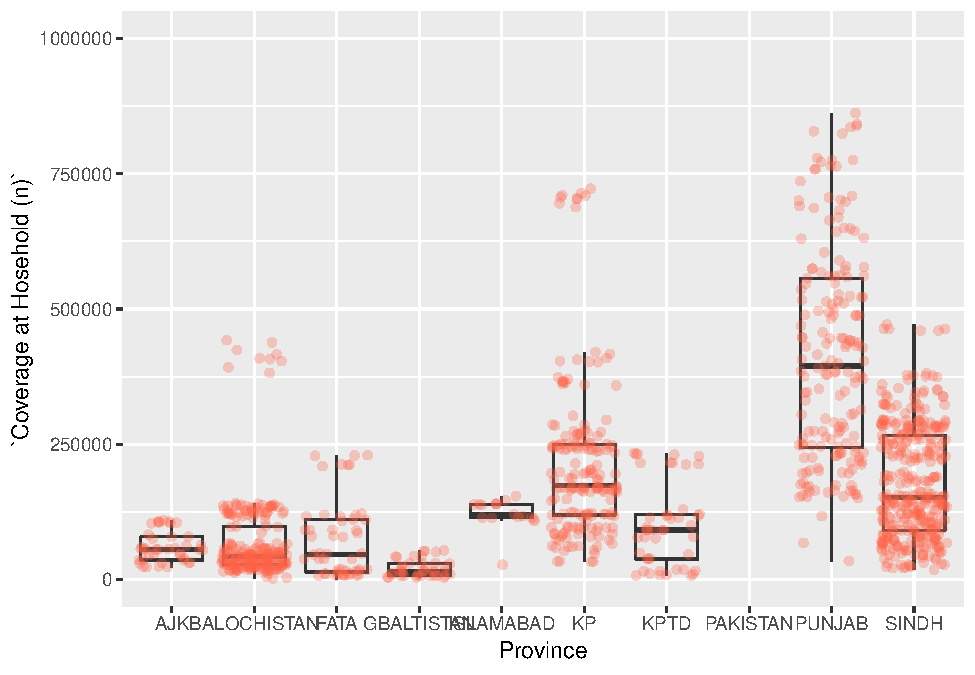
\includegraphics{M_E-plots-in-ggplot2_files/figure-latex/unnamed-chunk-11-1.pdf}

Finally, we will do some finishing touches.

\begin{Shaded}
\begin{Highlighting}[]
\NormalTok{plot5 <-}\StringTok{ }
\StringTok{  }\NormalTok{plot4 }\OperatorTok{+}
\StringTok{  }\KeywordTok{theme}\NormalTok{(}\DataTypeTok{axis.text.x =} \KeywordTok{element_text}\NormalTok{(}\DataTypeTok{angle =} \DecValTok{90}\NormalTok{, }\DataTypeTok{hjust =} \DecValTok{1}\NormalTok{)) }\OperatorTok{+}\StringTok{              }\CommentTok{# rotate the x-axis months label by 90 degrees}
\StringTok{  }\KeywordTok{scale_y_continuous}\NormalTok{(}\DataTypeTok{breaks =} \KeywordTok{round}\NormalTok{(}\KeywordTok{seq}\NormalTok{(}\KeywordTok{min}\NormalTok{(x}\OperatorTok{$}\NormalTok{cases), }\KeywordTok{max}\NormalTok{(x}\OperatorTok{$}\NormalTok{cases), }\DataTypeTok{by =} \DecValTok{50}\NormalTok{), }\DecValTok{1}\NormalTok{)) }\OperatorTok{+}\StringTok{ }\CommentTok{# add horizontal bold lines}
\StringTok{  }\KeywordTok{labs}\NormalTok{(}\DataTypeTok{caption =} \StringTok{"* Afp.rec Data as of  15-07-2019"}\NormalTok{) }\OperatorTok{+}\StringTok{                              }\CommentTok{# add a footnote}
\StringTok{  }\KeywordTok{theme}\NormalTok{(}
    \DataTypeTok{plot.caption =} \KeywordTok{element_text}\NormalTok{(}\DataTypeTok{size =} \DecValTok{7}\NormalTok{, }\DataTypeTok{face =} \StringTok{"italic"}\NormalTok{))                         }\CommentTok{# resize to small footnote}

\NormalTok{plot5}
\end{Highlighting}
\end{Shaded}

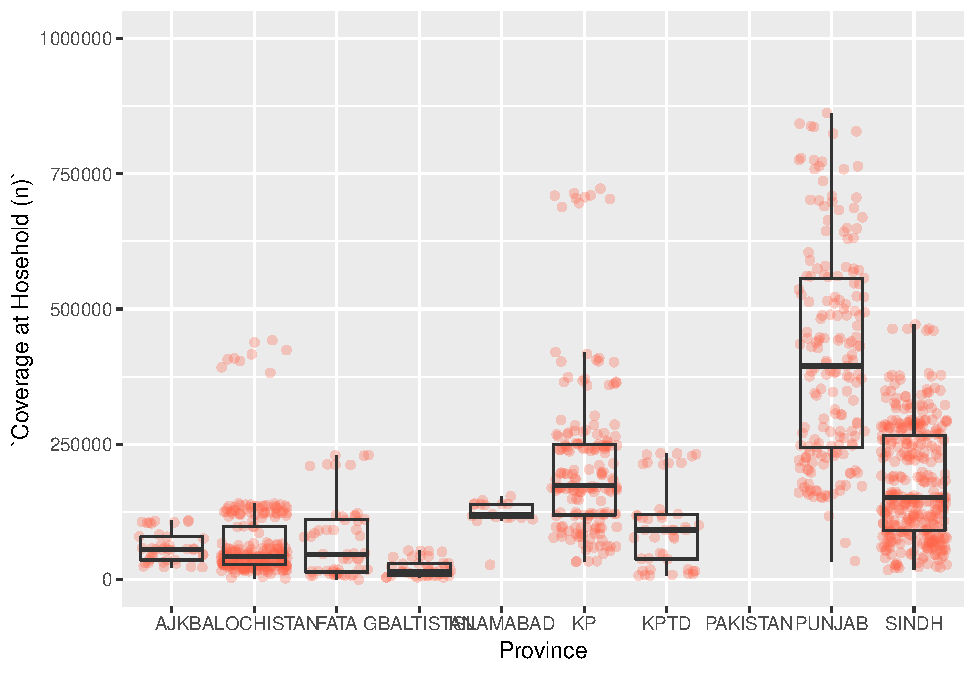
\includegraphics{M_E-plots-in-ggplot2_files/figure-latex/unnamed-chunk-12-1.pdf}

\hypertarget{environmental-sampling-results-2015-19-pakistan}{%
\subsubsection{Environmental Sampling Results 2015-19
Pakistan}\label{environmental-sampling-results-2015-19-pakistan}}

Read in the packages we will need.

\begin{Shaded}
\begin{Highlighting}[]
\KeywordTok{library}\NormalTok{(dplyr)}
\KeywordTok{library}\NormalTok{(zoo)}
\end{Highlighting}
\end{Shaded}

\begin{verbatim}
## Warning: package 'zoo' was built under R version 3.5.3
\end{verbatim}

\begin{verbatim}
## 
## Attaching package: 'zoo'
\end{verbatim}

\begin{verbatim}
## The following objects are masked from 'package:base':
## 
##     as.Date, as.Date.numeric
\end{verbatim}

\begin{Shaded}
\begin{Highlighting}[]
\KeywordTok{library}\NormalTok{(reshape2)}
\end{Highlighting}
\end{Shaded}

\begin{verbatim}
## Warning: package 'reshape2' was built under R version 3.5.3
\end{verbatim}

\begin{Shaded}
\begin{Highlighting}[]
\KeywordTok{library}\NormalTok{(ggplot2)}
\KeywordTok{library}\NormalTok{(scales)}
\end{Highlighting}
\end{Shaded}

\begin{verbatim}
## Warning: package 'scales' was built under R version 3.5.3
\end{verbatim}

\begin{Shaded}
\begin{Highlighting}[]
\KeywordTok{library}\NormalTok{(dataPakistan)}
\end{Highlighting}
\end{Shaded}

Load in the data \texttt{List\ of\ Env\ Samples\ 2015-2019.xlsx}.

\begin{Shaded}
\begin{Highlighting}[]
\NormalTok{file_name <-}\StringTok{ }\KeywordTok{system.file}\NormalTok{(}\DataTypeTok{package =} \StringTok{"dataPakistan"}\NormalTok{, }\StringTok{"extdata"}\NormalTok{, }\StringTok{"List of Env Samples 2015-2019.xlsx"}\NormalTok{)}

\CommentTok{# dat <- read_excel(file.choose())}
\NormalTok{dat <-}
\StringTok{  }\NormalTok{readxl}\OperatorTok{::}\KeywordTok{read_xlsx}\NormalTok{(}
    \DataTypeTok{path =}\NormalTok{ file_name,}
    \DataTypeTok{range =} \StringTok{"A2:F58"}\NormalTok{, }
    \DataTypeTok{sheet =} \StringTok{"Sheet1"}\NormalTok{) }\CommentTok{#, sheet = 1)}
\end{Highlighting}
\end{Shaded}

If we looks the \texttt{YRONSET} variable we see that only the first
month in a year has a value and the rest are empty (\texttt{NA}). We can
fill in the empty months by carrying forward the previous value.

\begin{Shaded}
\begin{Highlighting}[]
\CommentTok{##############}
\CommentTok{# preprocess #}
\CommentTok{##############}

\CommentTok{# fill in the empty year of onset}
\CommentTok{# last observation carried forward (LOCF)}
\NormalTok{dat}\OperatorTok{$}\NormalTok{YRONSET <-}\StringTok{ }\NormalTok{zoo}\OperatorTok{::}\KeywordTok{na.locf}\NormalTok{(dat}\OperatorTok{$}\NormalTok{YRONSET)}

\CommentTok{# check}
\NormalTok{dat}\OperatorTok{$}\NormalTok{YRONSET}
\end{Highlighting}
\end{Shaded}

\begin{verbatim}
##  [1] "2015"        "2015"        "2015"        "2015"        "2015"       
##  [6] "2015"        "2015"        "2015"        "2015"        "2015"       
## [11] "2015"        "2015"        "2016"        "2016"        "2016"       
## [16] "2016"        "2016"        "2016"        "2016"        "2016"       
## [21] "2016"        "2016"        "2016"        "2016"        "2017"       
## [26] "2017"        "2017"        "2017"        "2017"        "2017"       
## [31] "2017"        "2017"        "2017"        "2017"        "2017"       
## [36] "2017"        "2018"        "2018"        "2018"        "2018"       
## [41] "2018"        "2018"        "2018"        "2018"        "2018"       
## [46] "2018"        "2018"        "2018"        "2019"        "2019"       
## [51] "2019"        "2019"        "2019"        "2019"        "2019"       
## [56] "Grand Total"
\end{verbatim}

FOr each row (\texttt{rowwise}) we want to create a new value that tells
us whether the sum total of the Positive, Negative and Under Process
columns is the same as the Grand Total column. Call this new TRUE or
FALSE values \texttt{check\_total}.

To do this we can check for equivalence using the \texttt{==}.

\begin{Shaded}
\begin{Highlighting}[]
\NormalTok{dat <-}
\StringTok{  }\NormalTok{dat }\OperatorTok\StringTok{ }
\StringTok{  }\KeywordTok{rowwise}\NormalTok{() }\OperatorTok\StringTok{ }
\StringTok{  }\KeywordTok{mutate}\NormalTok{(}\DataTypeTok{check_total =} \KeywordTok{sum}\NormalTok{(Positive, Negative, }\StringTok{`}\DataTypeTok{Under Process}\StringTok{`}\NormalTok{, }\DataTypeTok{na.rm =} \OtherTok{TRUE}\NormalTok{) }\OperatorTok{==}\StringTok{ `}\DataTypeTok{Grand Total}\StringTok{`}\NormalTok{)}
\end{Highlighting}
\end{Shaded}

Now check to see if any of the rows do not have these things equal.

\begin{Shaded}
\begin{Highlighting}[]
\KeywordTok{any}\NormalTok{(}\OperatorTok{!}\NormalTok{dat}\OperatorTok{$}\NormalTok{check_total)}
\end{Highlighting}
\end{Shaded}

\begin{verbatim}
## [1] FALSE
\end{verbatim}

Looks ok! To keep things tidy lets remove the columns we won't need and
remove the last row which is a grand total.

\begin{Shaded}
\begin{Highlighting}[]
\NormalTok{dat <-}\StringTok{ }\NormalTok{dat }\OperatorTok\StringTok{ }\KeywordTok{select}\NormalTok{(}\OperatorTok{-}\StringTok{"Grand Total"}\NormalTok{, }\OperatorTok{-}\NormalTok{check_total)}
\NormalTok{dat <-}\StringTok{ }\NormalTok{dat[}\OperatorTok{-}\KeywordTok{nrow}\NormalTok{(dat), ]}
\end{Highlighting}
\end{Shaded}

Create a new combined month and year of onset column and make sure the
order is in calendar time.

\begin{Shaded}
\begin{Highlighting}[]
\NormalTok{dat}\OperatorTok{$}\NormalTok{month_year <-}\StringTok{ }\KeywordTok{paste}\NormalTok{(dat}\OperatorTok{$}\NormalTok{MONTH, dat}\OperatorTok{$}\NormalTok{YRONSET)}
\CommentTok{# dat$month <- factor(dat$month, ordered = TRUE)}
\NormalTok{dat}\OperatorTok{$}\NormalTok{month_year <-}\StringTok{ }\KeywordTok{factor}\NormalTok{(dat}\OperatorTok{$}\NormalTok{month_year, }\DataTypeTok{levels =}\NormalTok{ dat}\OperatorTok{$}\NormalTok{month_year, }\DataTypeTok{ordered =} \OtherTok{TRUE}\NormalTok{)}
\end{Highlighting}
\end{Shaded}

Finally, we need to reshape the data to the format that \texttt{ggplot2}
is expecting. To do this we will \texttt{melt} the data frame which
means to transform it to a long array, where there is one column for the
variable (\texttt{Positive}, \texttt{Negative}, \texttt{Under\ Process})
and one column for the corresponding value.

\begin{Shaded}
\begin{Highlighting}[]
\KeywordTok{library}\NormalTok{(reshape2)}

\NormalTok{x <-}\StringTok{ }\KeywordTok{melt}\NormalTok{(dat, }\DataTypeTok{id.vars =} \KeywordTok{c}\NormalTok{(}\StringTok{"YRONSET"}\NormalTok{, }\StringTok{"MONTH"}\NormalTok{, }\StringTok{"month_year"}\NormalTok{))}
\NormalTok{x}\OperatorTok{$}\NormalTok{variable <-}\StringTok{ }\KeywordTok{factor}\NormalTok{(x}\OperatorTok{$}\NormalTok{variable,}
                     \DataTypeTok{levels =} \KeywordTok{c}\NormalTok{(}\StringTok{"Positive"}\NormalTok{, }\StringTok{"Negative"}\NormalTok{, }\StringTok{"Under Process"}\NormalTok{))}

\CommentTok{# put Negative first in the ordering}
\NormalTok{x}\OperatorTok{$}\NormalTok{variable <-}\StringTok{ }\KeywordTok{relevel}\NormalTok{(x}\OperatorTok{$}\NormalTok{variable, }\StringTok{'Negative'}\NormalTok{)}
\end{Highlighting}
\end{Shaded}

\begin{Shaded}
\begin{Highlighting}[]
\CommentTok{#########}
\CommentTok{# plots #}
\CommentTok{#########}


\CommentTok{# basic stacked bar plot}
\NormalTok{plot0 <-}
\StringTok{  }\KeywordTok{ggplot}\NormalTok{(x, }\KeywordTok{aes}\NormalTok{(}\DataTypeTok{x =}\NormalTok{ month_year, }\DataTypeTok{y =}\NormalTok{ value, }\DataTypeTok{fill =}\NormalTok{ variable)) }\OperatorTok{+}
\StringTok{  }\KeywordTok{geom_bar}\NormalTok{(}\DataTypeTok{position =} \StringTok{"fill"}\NormalTok{, }\DataTypeTok{stat =} \StringTok{"identity"}\NormalTok{)}

\NormalTok{plot0}
\end{Highlighting}
\end{Shaded}

\begin{verbatim}
## Warning: Removed 55 rows containing missing values (position_stack).
\end{verbatim}

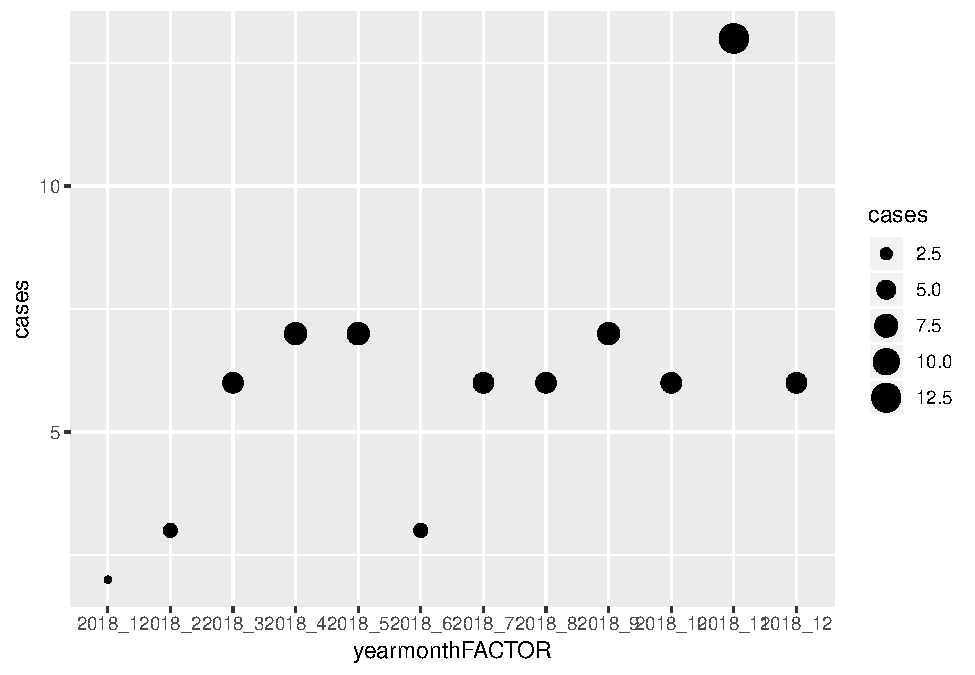
\includegraphics{M_E-plots-in-ggplot2_files/figure-latex/unnamed-chunk-21-1.pdf}

\begin{Shaded}
\begin{Highlighting}[]
\KeywordTok{library}\NormalTok{(scales)}

\NormalTok{plot1 <-}\StringTok{ }
\StringTok{  }\NormalTok{plot0 }\OperatorTok{+}
\StringTok{  }\KeywordTok{scale_fill_manual}\NormalTok{(}\StringTok{"legend"}\NormalTok{,}
                    \DataTypeTok{values =} \KeywordTok{c}\NormalTok{(}\StringTok{"Negative"}\NormalTok{ =}\StringTok{ "lightgreen"}\NormalTok{,         }\CommentTok{# change the colour scheme}
                               \StringTok{"Positive"}\NormalTok{ =}\StringTok{ "red"}\NormalTok{,}
                               \StringTok{"Under Process"}\NormalTok{ =}\StringTok{ "grey"}\NormalTok{)) }\OperatorTok{+}
\StringTok{  }\KeywordTok{scale_y_continuous}\NormalTok{(}\DataTypeTok{labels =} \KeywordTok{percent_format}\NormalTok{(),}
                     \DataTypeTok{breaks =} \KeywordTok{seq}\NormalTok{(}\DataTypeTok{from =} \DecValTok{0}\NormalTok{, }\DataTypeTok{to =} \DecValTok{1}\NormalTok{, }\DataTypeTok{by =} \FloatTok{0.1}\NormalTok{)) }\OperatorTok{+}\StringTok{  }\CommentTok{# change y-axis labels to %s}
\StringTok{  }\KeywordTok{scale_x_discrete}\NormalTok{(}\DataTypeTok{breaks =}\NormalTok{ x}\OperatorTok{$}\NormalTok{month_year, }\DataTypeTok{labels =}\NormalTok{ x}\OperatorTok{$}\NormalTok{MONTH,}
                   \DataTypeTok{expand =} \KeywordTok{c}\NormalTok{(}\FloatTok{0.1}\NormalTok{,}\FloatTok{0.1}\NormalTok{)) }\OperatorTok{+}
\StringTok{  }\KeywordTok{facet_grid}\NormalTok{(}\OperatorTok{~}\StringTok{ }\NormalTok{YRONSET, }\DataTypeTok{space =} \StringTok{"free_x"}\NormalTok{, }\DataTypeTok{scales =} \StringTok{"free_x"}\NormalTok{, }\DataTypeTok{switch =} \StringTok{"x"}\NormalTok{) }\OperatorTok{+}\StringTok{  }\CommentTok{# separate into years}
\StringTok{  }\KeywordTok{theme_bw}\NormalTok{() }\OperatorTok{+}\StringTok{                                                                }\CommentTok{# black and white theme}
\StringTok{  }\KeywordTok{theme}\NormalTok{(}\DataTypeTok{strip.placement =} \StringTok{"outside"}\NormalTok{,}
        \DataTypeTok{strip.background =} \KeywordTok{element_rect}\NormalTok{(}\DataTypeTok{fill =} \OtherTok{NA}\NormalTok{, }\DataTypeTok{colour =} \StringTok{"green"}\NormalTok{),    }\CommentTok{# swap x-axis labels, recolour}
        \DataTypeTok{panel.spacing =} \KeywordTok{unit}\NormalTok{(}\DecValTok{0}\NormalTok{,}\StringTok{"cm"}\NormalTok{)) }\OperatorTok{+}
\StringTok{  }\KeywordTok{ggtitle}\NormalTok{(}\StringTok{"Environmental Sampling Results 2015-19* }\CharTok{\textbackslash{}n}\StringTok{Pakistan"}\NormalTok{) }\OperatorTok{+}
\StringTok{  }\KeywordTok{theme}\NormalTok{(}\DataTypeTok{axis.text.x =} \KeywordTok{element_text}\NormalTok{(}\DataTypeTok{angle =} \DecValTok{90}\NormalTok{, }\DataTypeTok{hjust =} \DecValTok{1}\NormalTok{))}
\end{Highlighting}
\end{Shaded}

We want to move the legend to below the plot.

\begin{Shaded}
\begin{Highlighting}[]
\NormalTok{plot2 <-}\StringTok{ }
\StringTok{  }\NormalTok{plot1 }\OperatorTok{+}
\StringTok{  }\KeywordTok{xlab}\NormalTok{(}\StringTok{""}\NormalTok{) }\OperatorTok{+}\StringTok{ }\KeywordTok{ylab}\NormalTok{(}\StringTok{""}\NormalTok{) }\OperatorTok{+}
\StringTok{  }\KeywordTok{theme}\NormalTok{(}\DataTypeTok{legend.position =} \StringTok{"bottom"}\NormalTok{, }\DataTypeTok{legend.title =} \KeywordTok{element_blank}\NormalTok{())}
\end{Highlighting}
\end{Shaded}

Finally, annotate the bars with their values.

\begin{Shaded}
\begin{Highlighting}[]
\NormalTok{plot3 <-}\StringTok{ }
\StringTok{  }\NormalTok{plot2 }\OperatorTok{+}
\StringTok{  }\KeywordTok{geom_text}\NormalTok{(}\DataTypeTok{data =}\NormalTok{ x, }\KeywordTok{aes}\NormalTok{(}\DataTypeTok{y =}\NormalTok{ value, }\DataTypeTok{label =}\NormalTok{ value), }\DataTypeTok{position =} \KeywordTok{position_fill}\NormalTok{(}\DataTypeTok{vjust =} \FloatTok{0.5}\NormalTok{))}

\NormalTok{plot3}
\end{Highlighting}
\end{Shaded}

\begin{verbatim}
## Warning: Removed 55 rows containing missing values (position_stack).

## Warning: Removed 55 rows containing missing values (position_stack).
\end{verbatim}

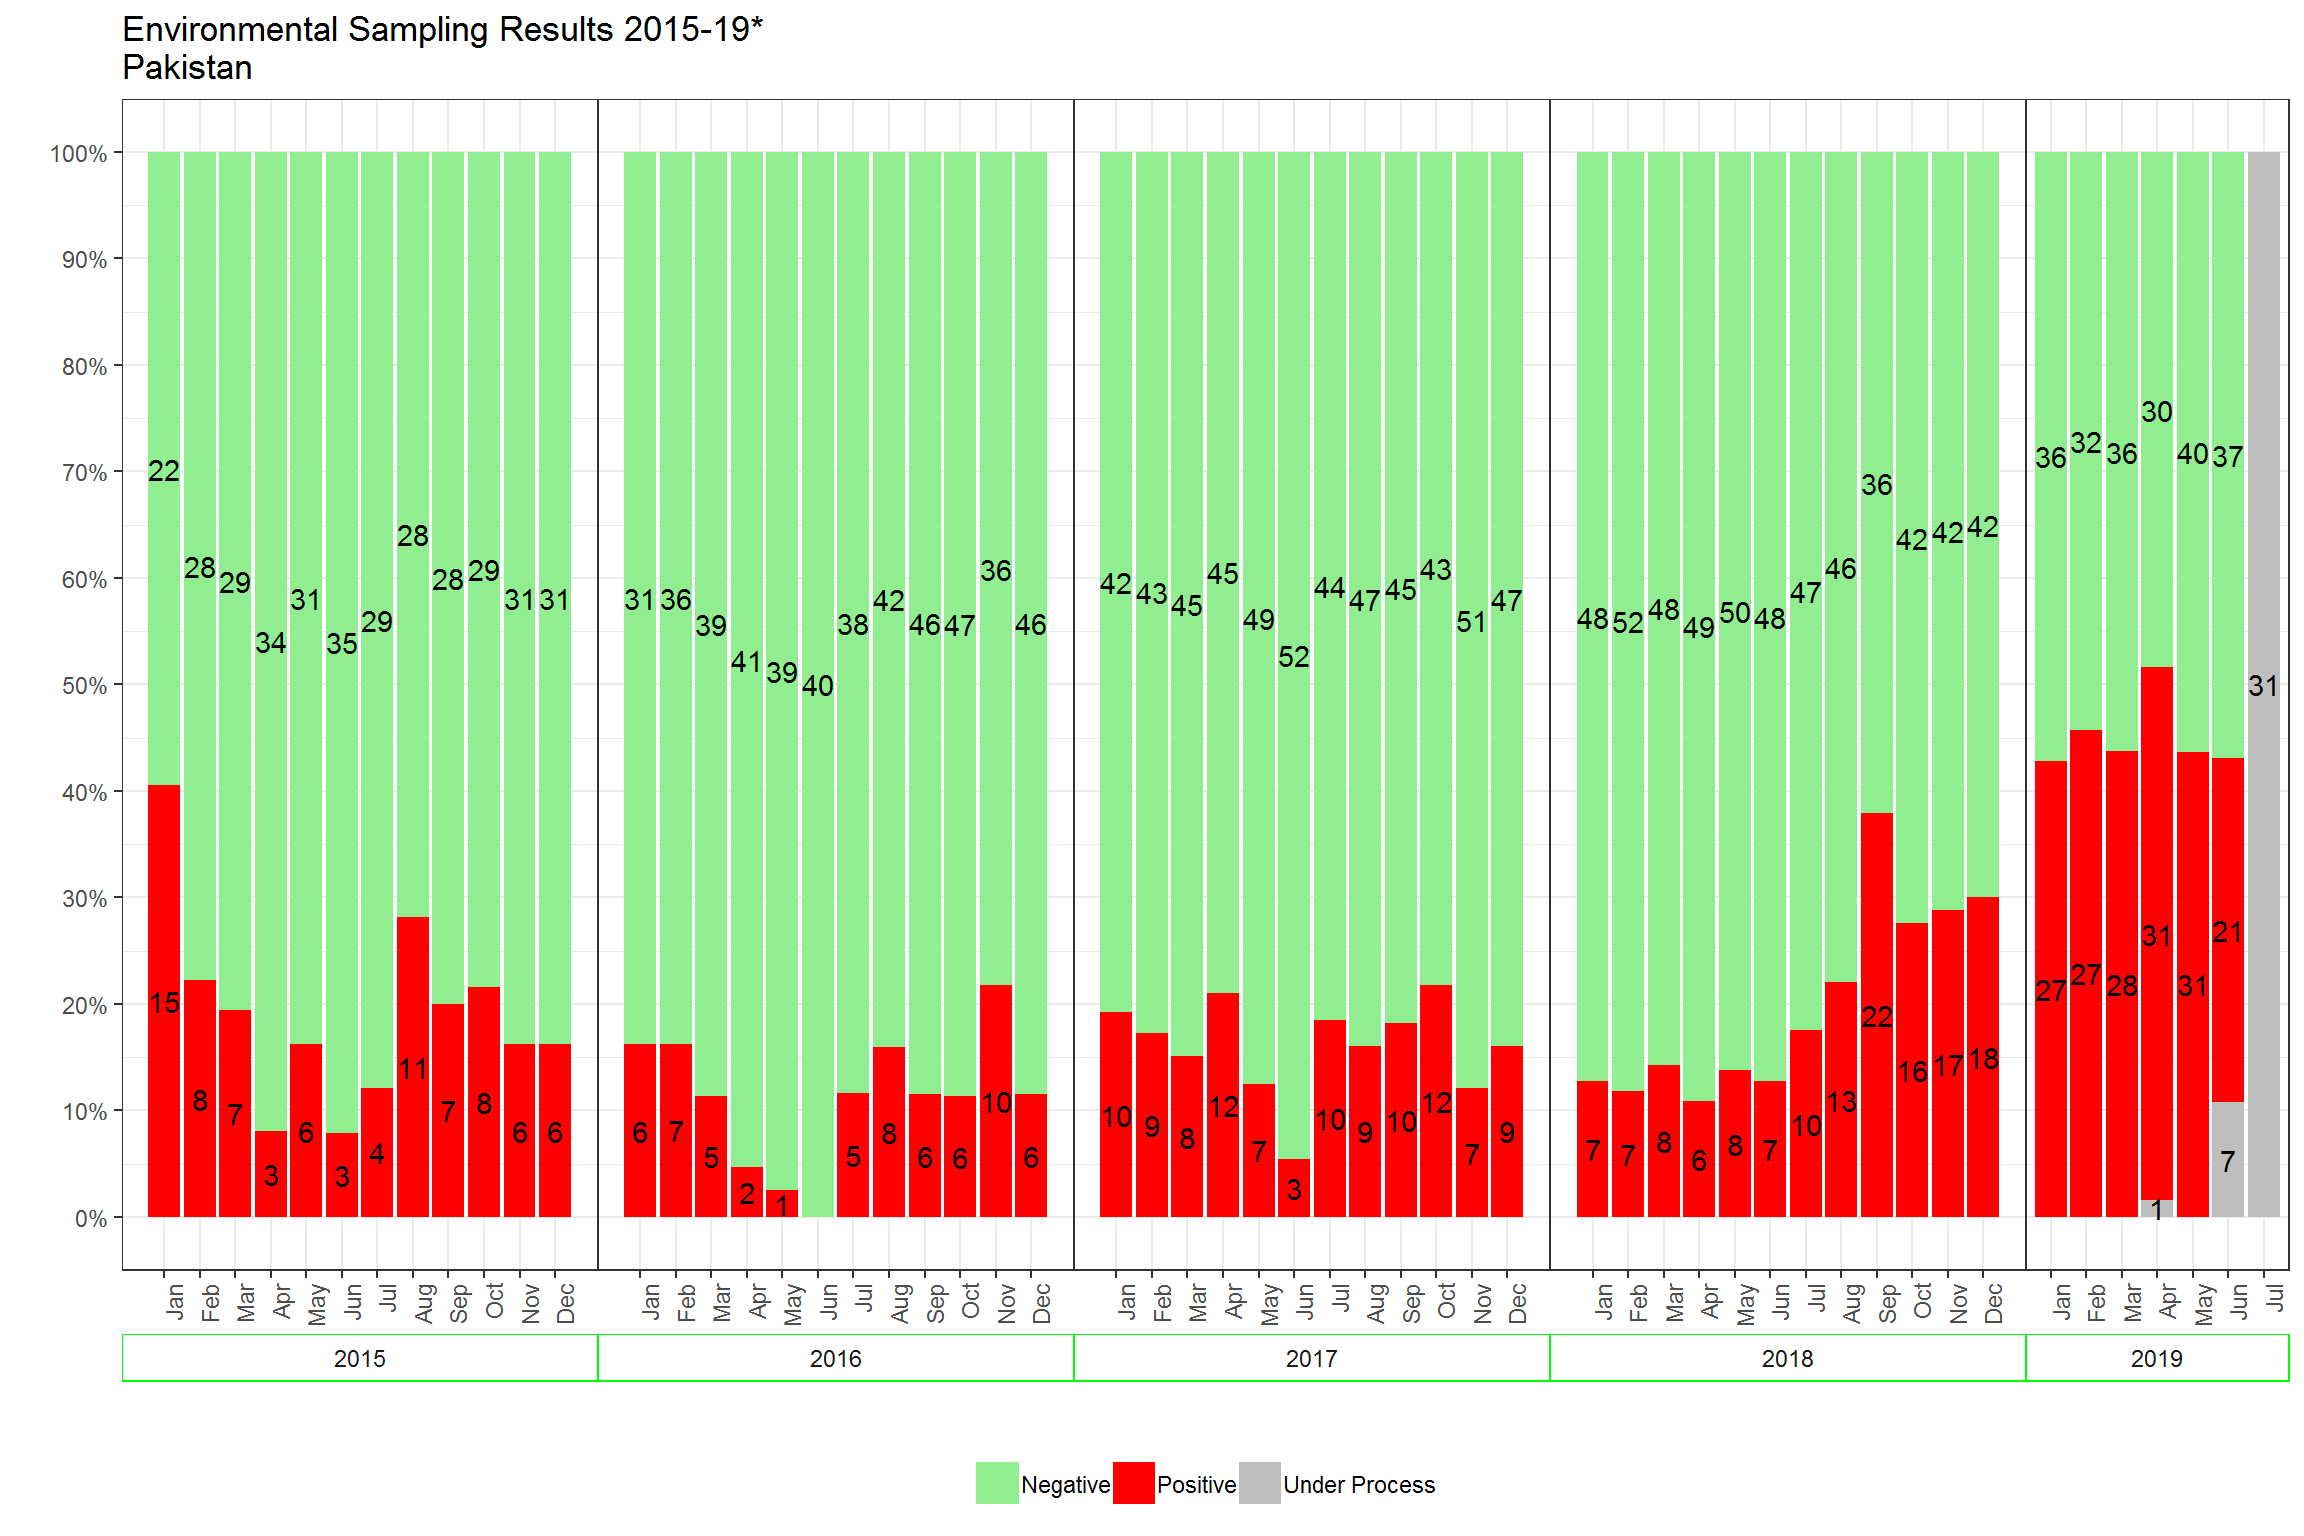
\includegraphics{M_E-plots-in-ggplot2_files/figure-latex/unnamed-chunk-24-1.pdf}

\hypertarget{mpqa-_march-snid}{%
\subsubsection{MPQA \_March SNID}\label{mpqa-_march-snid}}

Load packages.

\begin{Shaded}
\begin{Highlighting}[]
\KeywordTok{library}\NormalTok{(dplyr)}
\KeywordTok{library}\NormalTok{(zoo)}
\KeywordTok{library}\NormalTok{(reshape2)}
\KeywordTok{library}\NormalTok{(ggplot2)}
\KeywordTok{library}\NormalTok{(scales)}

\KeywordTok{library}\NormalTok{(dataPakistan)}
\end{Highlighting}
\end{Shaded}

Load in data.

\begin{Shaded}
\begin{Highlighting}[]
\NormalTok{file_name <-}\StringTok{ }\KeywordTok{system.file}\NormalTok{(}\DataTypeTok{package =} \StringTok{"dataPakistan"}\NormalTok{, }\StringTok{"extdata"}\NormalTok{, }\StringTok{"MPQA _March SNID.xlsx"}\NormalTok{)}
\NormalTok{dat <-}\StringTok{ }\NormalTok{readxl}\OperatorTok{::}\KeywordTok{read_xlsx}\NormalTok{(file_name)}
\end{Highlighting}
\end{Shaded}

\begin{Shaded}
\begin{Highlighting}[]
\CommentTok{##############}
\CommentTok{# preprocess #}
\CommentTok{##############}

\CommentTok{# remove columns we dont need}
\NormalTok{x <-}\StringTok{ }\NormalTok{dat }\OperatorTok\StringTok{ }\KeywordTok{select}\NormalTok{(}\OperatorTok{-}\NormalTok{DESK, }\OperatorTok{-}\NormalTok{FIELD)}

\CommentTok{# create a Province-Ditrict single string}
\NormalTok{x}\OperatorTok{$}\NormalTok{prov_district <-}\StringTok{ }\KeywordTok{paste}\NormalTok{(x}\OperatorTok{$}\StringTok{"Province name"}\NormalTok{, x}\OperatorTok{$}\StringTok{"District name"}\NormalTok{)}
\end{Highlighting}
\end{Shaded}

\begin{Shaded}
\begin{Highlighting}[]
\CommentTok{#########}
\CommentTok{# plots #}
\CommentTok{#########}

\CommentTok{# basic plot}
\NormalTok{plot0 <-}\StringTok{ }
\StringTok{  }\KeywordTok{ggplot}\NormalTok{(x, }\KeywordTok{aes}\NormalTok{(}\DataTypeTok{x =}\NormalTok{ prov_district, }\DataTypeTok{y =}\NormalTok{ Overall)) }\OperatorTok{+}
\StringTok{  }\KeywordTok{geom_bar}\NormalTok{(}\DataTypeTok{stat =} \StringTok{"identity"}\NormalTok{, }\DataTypeTok{fill =} \StringTok{"lightgreen"}\NormalTok{)}

\NormalTok{plot0}
\end{Highlighting}
\end{Shaded}

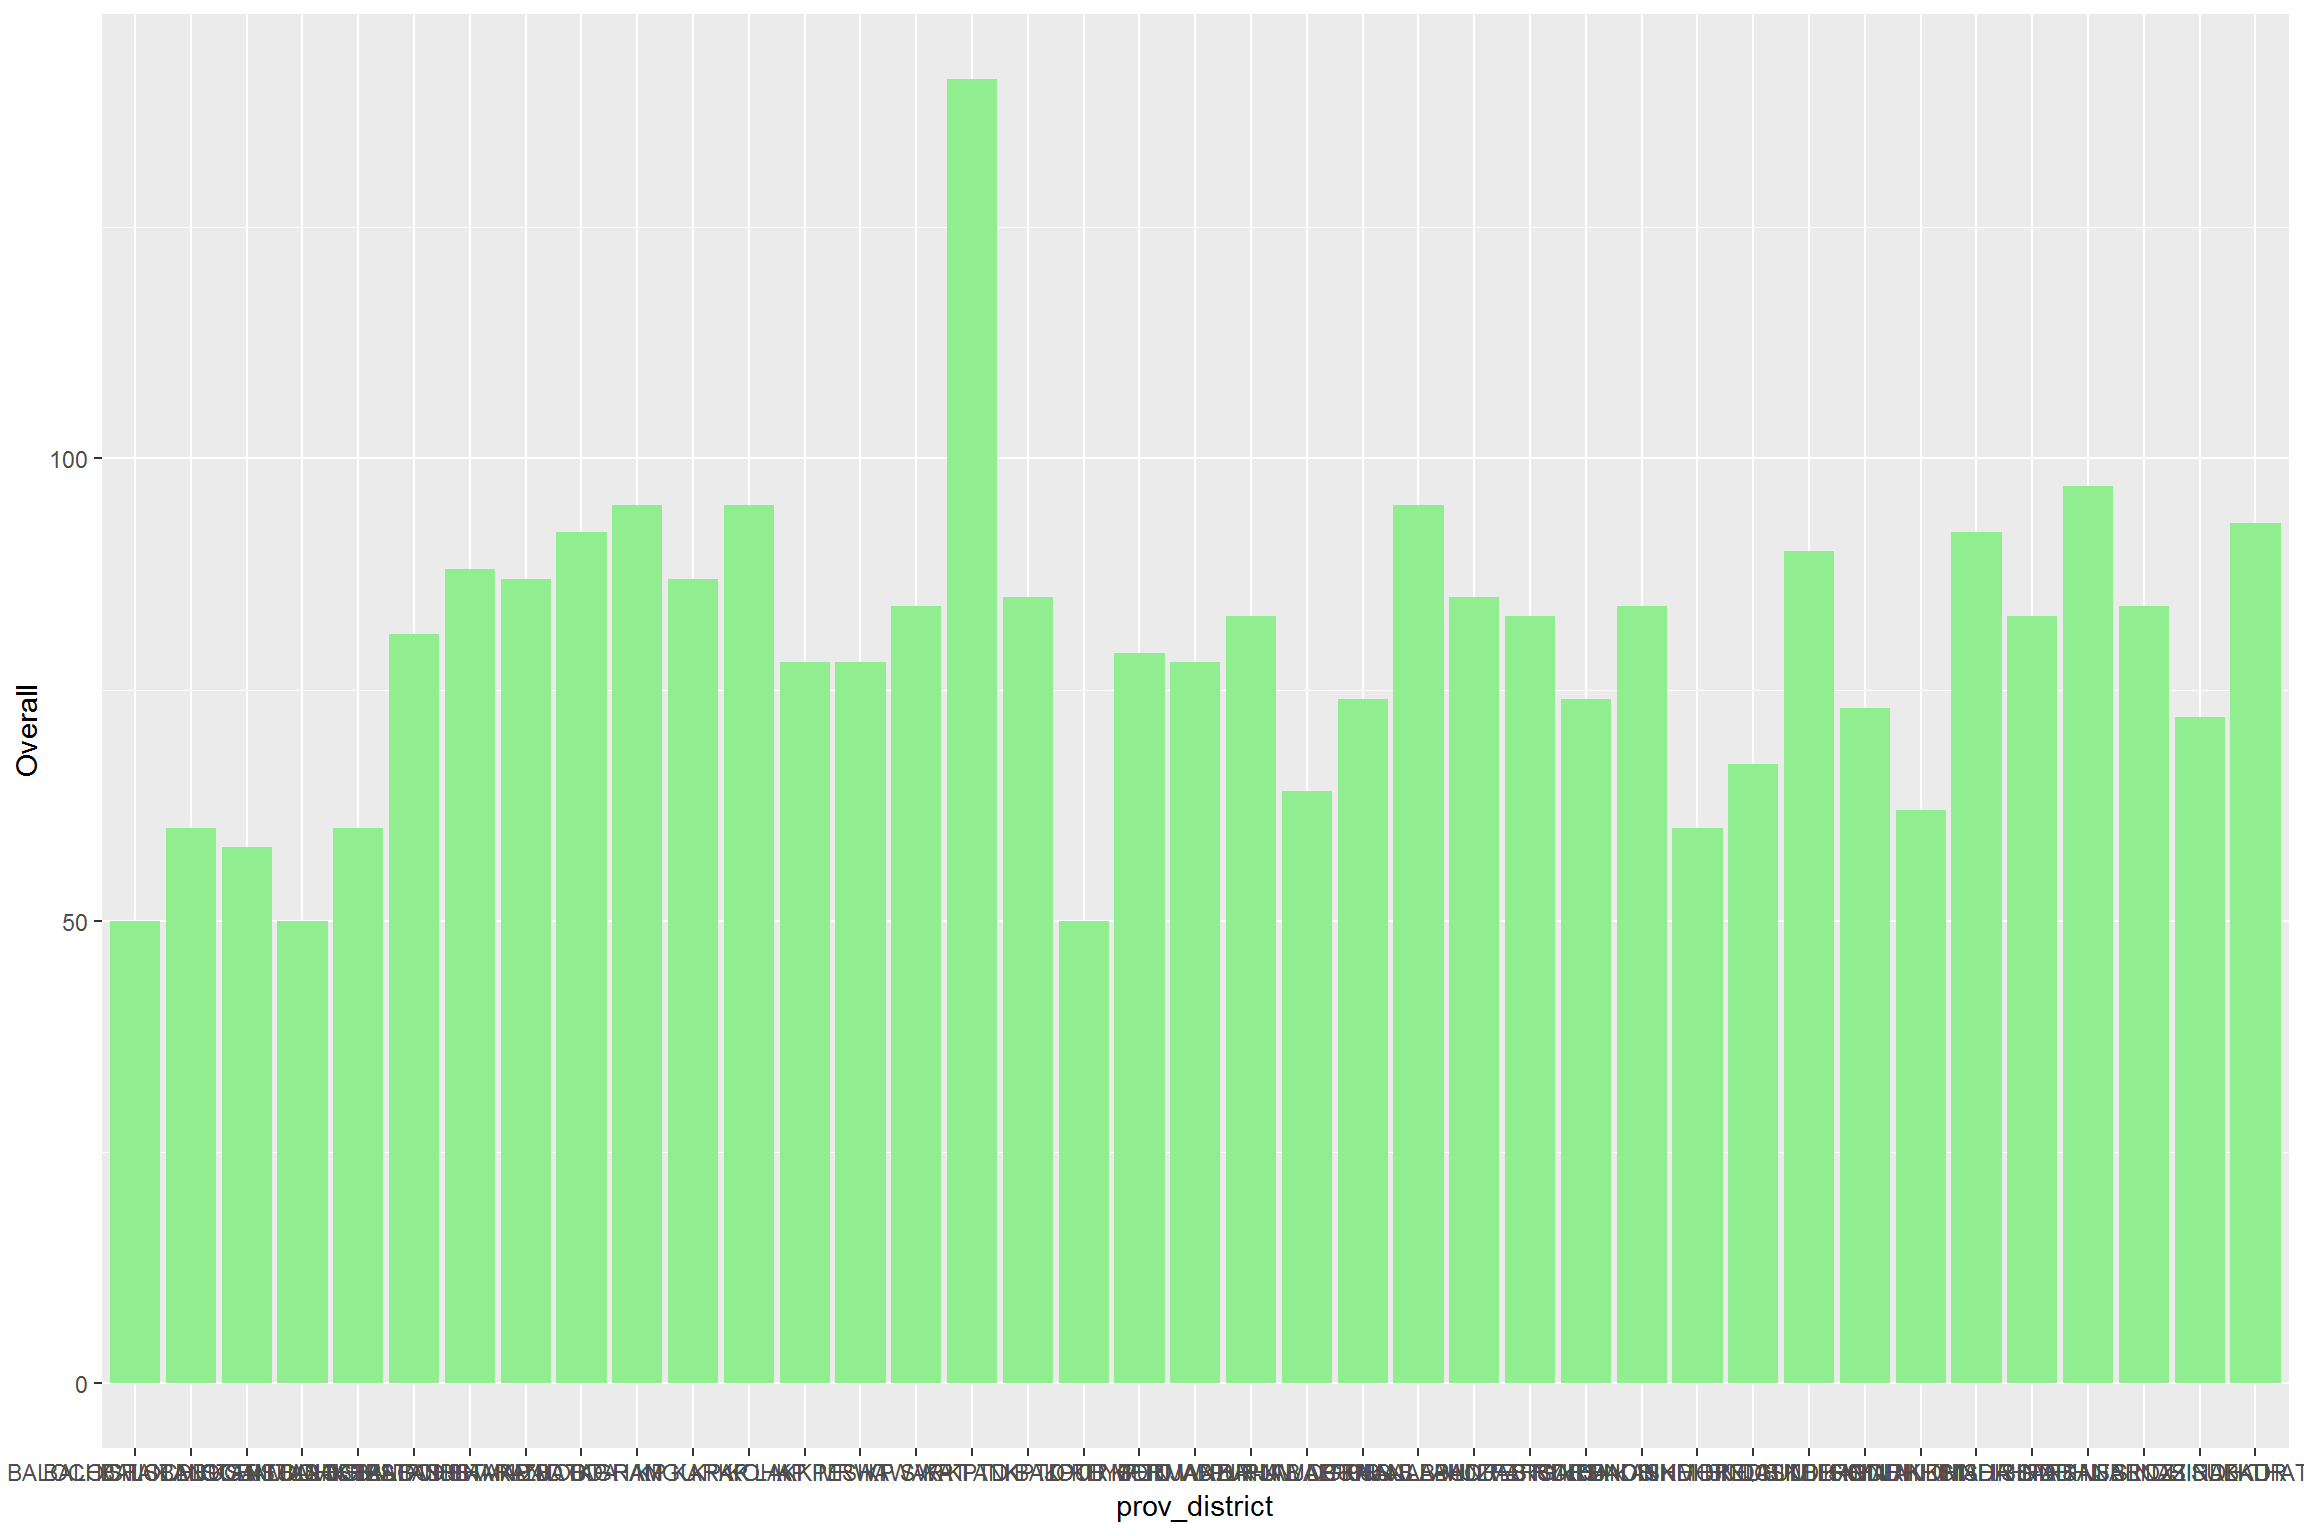
\includegraphics{M_E-plots-in-ggplot2_files/figure-latex/unnamed-chunk-28-1.pdf}

\begin{Shaded}
\begin{Highlighting}[]
\NormalTok{plot1 <-}\StringTok{ }
\StringTok{  }\NormalTok{plot0 }\OperatorTok{+}
\StringTok{  }\KeywordTok{geom_text}\NormalTok{(}\KeywordTok{aes}\NormalTok{(}\DataTypeTok{label =} \KeywordTok{sprintf}\NormalTok{(}\StringTok{"%d%%"}\NormalTok{, Overall)), }\DataTypeTok{vjust =} \DecValTok{0}\NormalTok{, }\DataTypeTok{angle =} \DecValTok{-90}\NormalTok{, }\DataTypeTok{nudge_y =} \DecValTok{-5}\NormalTok{) }\OperatorTok{+}
\StringTok{  }\KeywordTok{scale_x_discrete}\NormalTok{(}\DataTypeTok{breaks =}\NormalTok{ x}\OperatorTok{$}\NormalTok{prov_district, }\DataTypeTok{labels =}\NormalTok{ x}\OperatorTok{$}\StringTok{"District name"}\NormalTok{,}
                   \DataTypeTok{expand =} \KeywordTok{c}\NormalTok{(}\FloatTok{0.1}\NormalTok{,}\FloatTok{0.1}\NormalTok{)) }\OperatorTok{+}
\StringTok{  }\KeywordTok{facet_grid}\NormalTok{(}\OperatorTok{~}\StringTok{ `}\DataTypeTok{Province name}\StringTok{`}\NormalTok{, }\DataTypeTok{space =} \StringTok{"free_x"}\NormalTok{, }\DataTypeTok{scales =} \StringTok{"free_x"}\NormalTok{, }\DataTypeTok{switch =} \StringTok{"x"}\NormalTok{) }\OperatorTok{+}\StringTok{ }
\StringTok{  }\KeywordTok{theme_bw}\NormalTok{() }\OperatorTok{+}
\StringTok{  }\KeywordTok{theme}\NormalTok{(}\DataTypeTok{strip.placement =} \StringTok{"outside"}\NormalTok{,}
        \DataTypeTok{strip.background =} \KeywordTok{element_rect}\NormalTok{(}\DataTypeTok{fill =} \OtherTok{NA}\NormalTok{, }\DataTypeTok{linetype =} \DecValTok{0}\NormalTok{),}
        \DataTypeTok{plot.title =} \KeywordTok{element_text}\NormalTok{(}\DataTypeTok{hjust =} \FloatTok{0.5}\NormalTok{, }\DataTypeTok{face =} \StringTok{"bold"}\NormalTok{),}
        \DataTypeTok{panel.spacing =} \KeywordTok{unit}\NormalTok{(}\DecValTok{0}\NormalTok{,}\StringTok{"cm"}\NormalTok{)) }\OperatorTok{+}
\StringTok{  }\KeywordTok{labs}\NormalTok{(}\DataTypeTok{subtitle =}
         \StringTok{"- Micro Plans of Tier-1 Districts from Karachi town, Quetta Block and Peshawar/Khyber are passed}\CharTok{\textbackslash{}n}\StringTok{- Substantial gaps identified primarily in Balochistan and pockets of KP and Sindh"}\NormalTok{) }\OperatorTok{+}
\StringTok{  }\KeywordTok{ggtitle}\NormalTok{(}\StringTok{"SUMMARY OF MPQA RESULTS"}\NormalTok{, ) }\OperatorTok{+}
\StringTok{  }\KeywordTok{xlab}\NormalTok{(}\StringTok{""}\NormalTok{) }\OperatorTok{+}\StringTok{ }\KeywordTok{ylab}\NormalTok{(}\StringTok{""}\NormalTok{) }\OperatorTok{+}\StringTok{ }\KeywordTok{theme}\NormalTok{(}\DataTypeTok{axis.text.x =} \KeywordTok{element_text}\NormalTok{(}\DataTypeTok{angle =} \DecValTok{90}\NormalTok{, }\DataTypeTok{hjust =} \DecValTok{1}\NormalTok{))}

\NormalTok{plot1}
\end{Highlighting}
\end{Shaded}

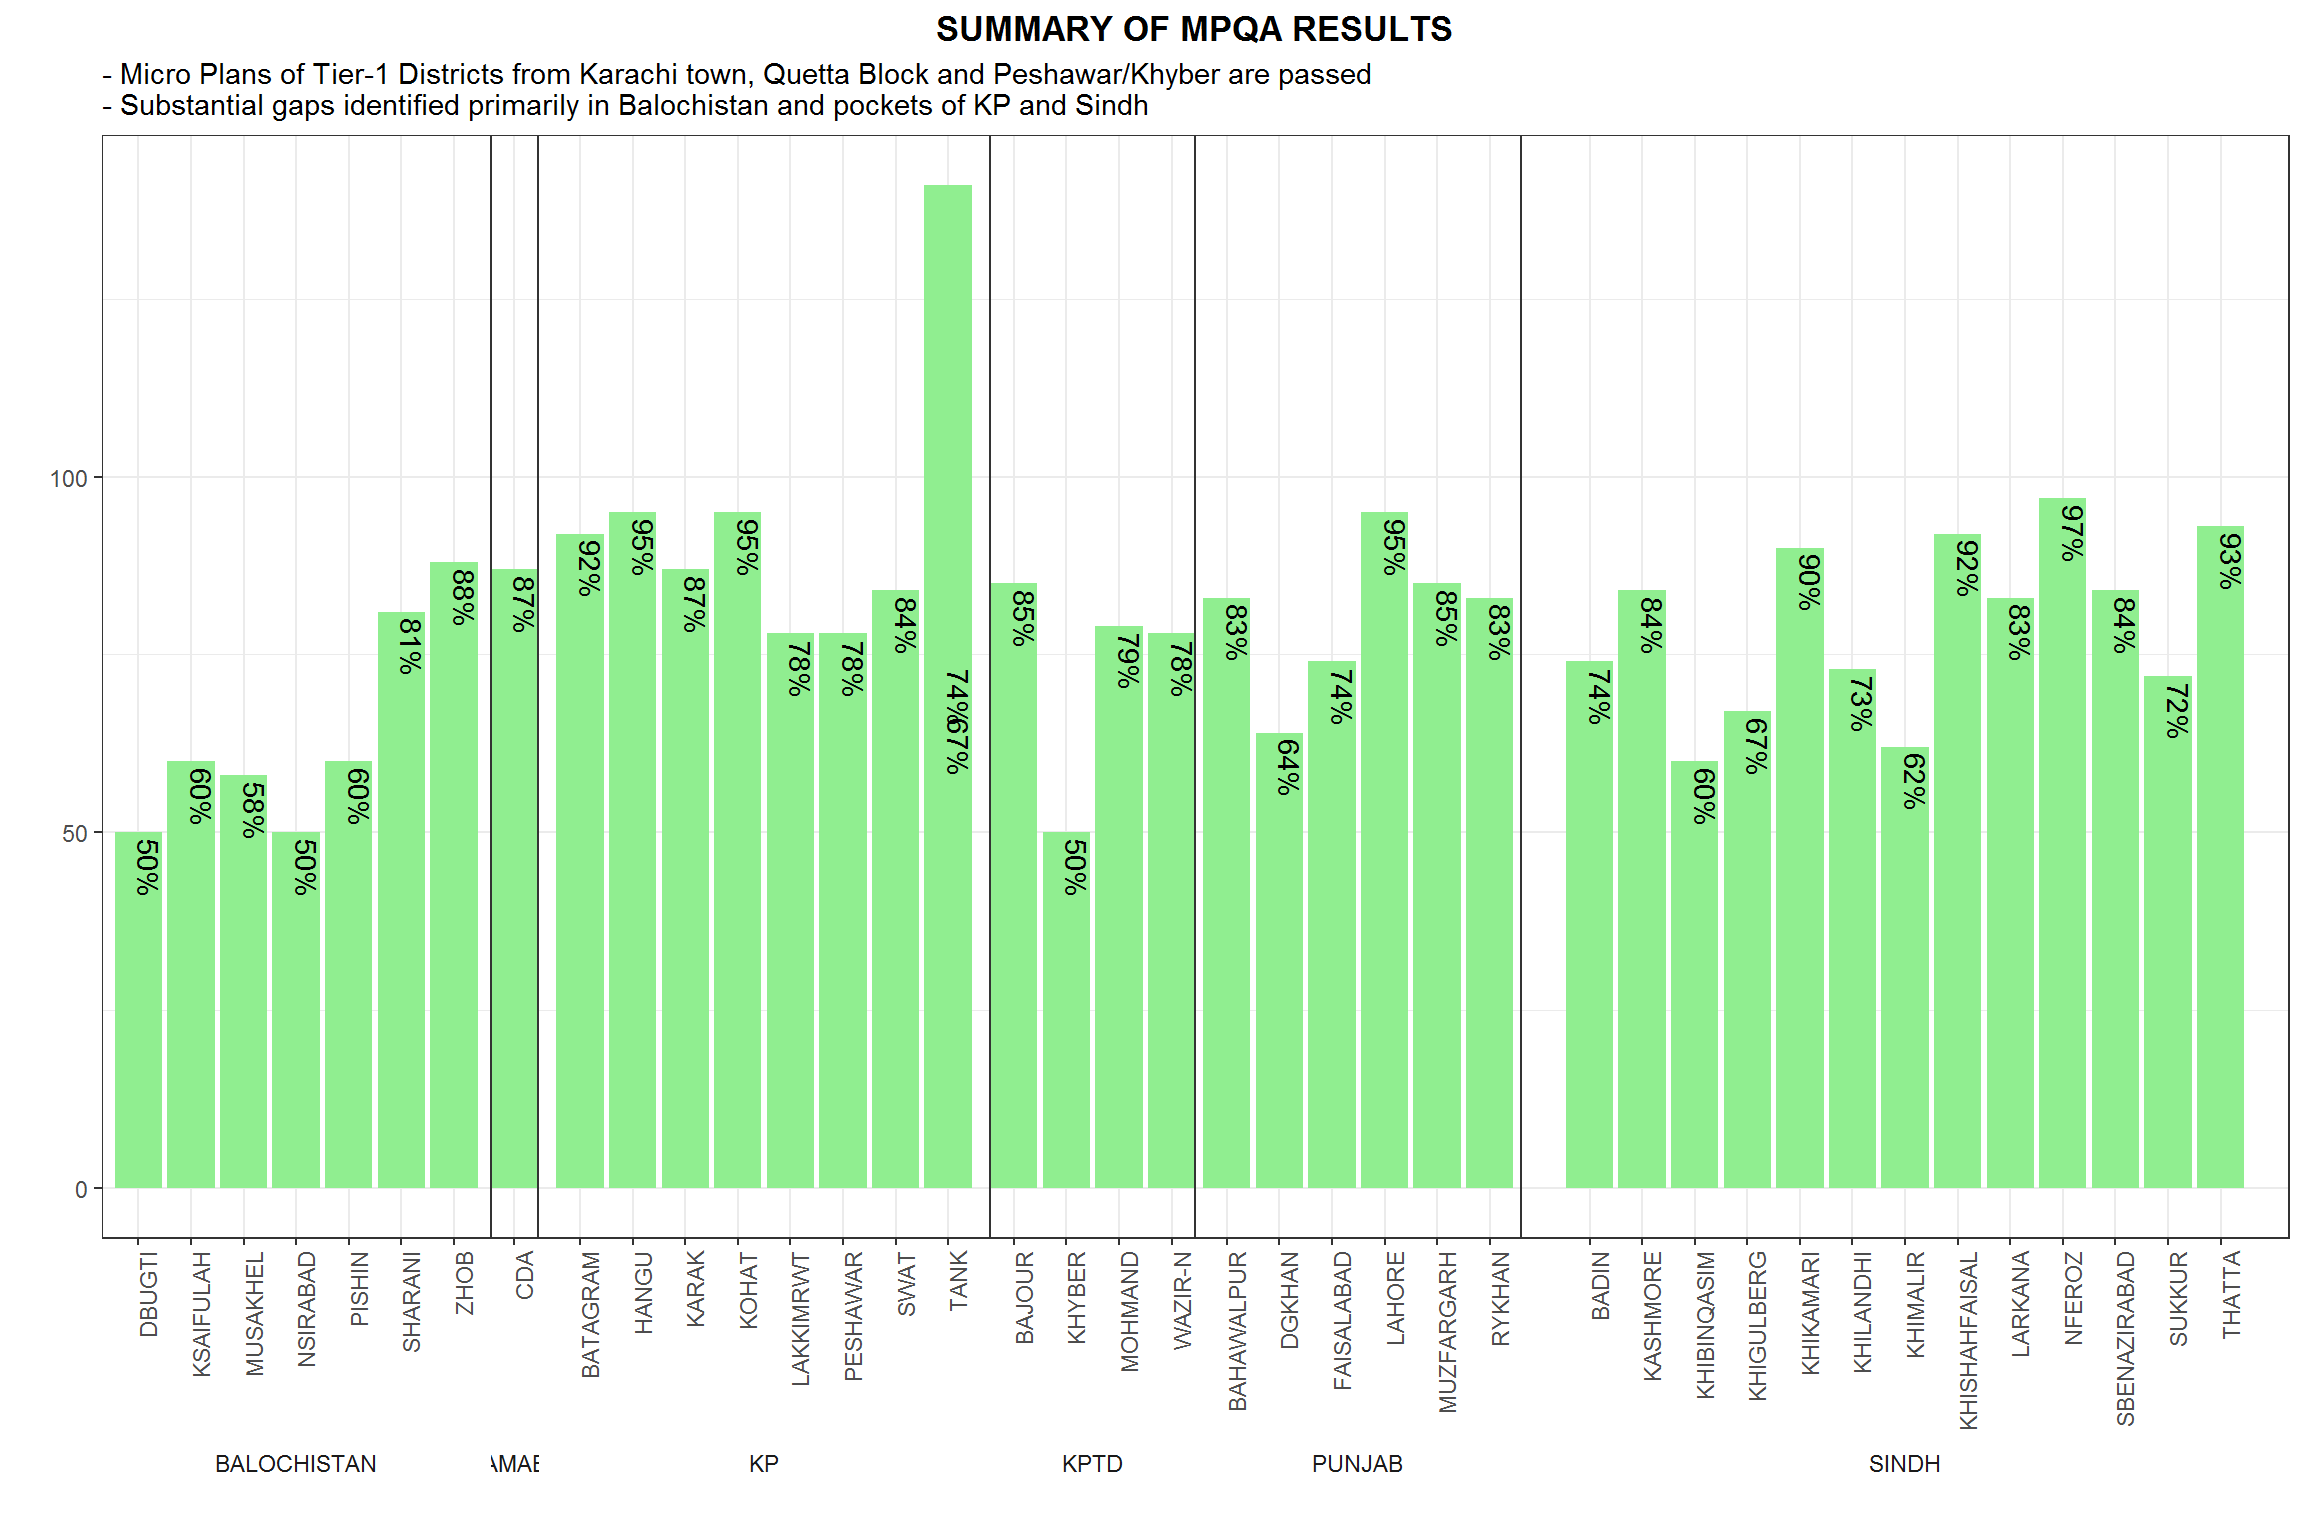
\includegraphics{M_E-plots-in-ggplot2_files/figure-latex/unnamed-chunk-29-1.pdf}


\end{document}
